
\chapter{Results}
\label{sec:org82a161d}

In this chapter the simulation results are presented with reference to the aim of the thesis, which was to study the mapping metrics.
Their precision when assessing the mapping quality and their relation with the error amount after mapping.
First, in the \hyperref[sec:org28dbcca]{Impact of mapping in the overall circuit error} section we show how the mapping procedure affects the general increment of error.
After that, we analyze the metrics and their correlation with the error increase in the \hyperref[sec:org2c64a48]{Analysis of the mapping metrics} section.

\section{Impact of mapping in the overall circuit error}
\label{sec:org28dbcca}
After the selection of benchmarks in the \href{chapter-4.org}{Benchmarks} section, we started their simulations with the simulation framework.
Not surprisingly, some of the benchmarks either had very long simulation times or were even impossible to simulate in our lab servers.
In most of those cases the circuits had more than ten qubits.
As we mentioned before throughout this thesis, the simulation of quantum systems is computationally exhausting.
As the number of qubits or the longitude of the circuit increase, the harder is to simulate them.
Indeed, it is a critical issue in our case, as soon as we need to run multiple simulations in a complex error model.
Therefore, as it can be seen in Tab. \ref{tab:map_selected_benchs}, we address that the final benchmark selection has a limitation in the number of qubits.

\begin{table}[htbp]
\caption{\label{tab:map_selected_benchs}
Table of the selected benchmarks to be mapped.}
\centering
\small
\begin{tabular}{lrrr}
\hline
Benchmark & \# qubits & \# gates & two-qubit gates (percentage)\\
\hline
4gt11\(_{\text{82}}\) & 5 & 27 & 0.667\\
4gt12\(_{\text{v1}}\)\(_{\text{89}}\) & 6 & 228 & 0.439\\
4gt4\(_{\text{v0}}\)\(_{\text{72}}\) & 6 & 258 & 0.438\\
4mod5\(_{\text{bdd}}\)\(_{\text{287}}\) & 7 & 70 & 0.443\\
4mod5\(_{\text{v0}}\)\(_{\text{20}}\) & 5 & 20 & 0.500\\
alu\(_{\text{bdd}}\)\(_{\text{288}}\) & 7 & 84 & 0.452\\
alu\(_{\text{v0}}\)\(_{\text{27}}\) & 5 & 36 & 0.472\\
decod24\(_{\text{bdd}}\)\(_{\text{294}}\) & 6 & 73 & 0.438\\
decod24\(_{\text{enable}}\)\(_{\text{126}}\) & 6 & 338 & 0.441\\
graycode6\(_{\text{47}}\) & 6 & 5 & 1.000\\
ham3\(_{\text{102}}\) & 3 & 20 & 0.550\\
hwb4\(_{\text{49}}\) & 5 & 233 & 0.459\\
mod10\(_{\text{176}}\) & 5 & 178 & 0.438\\
mod5adder\(_{\text{127}}\) & 6 & 555 & 0.431\\
mod5d1\(_{\text{63}}\) & 5 & 22 & 0.591\\
mod8\(_{\text{10}}\)\(_{\text{177}}\) & 6 & 440 & 0.445\\
one\(_{\text{two}}\)\(_{\text{three}}\)\(_{\text{v1}}\)\(_{\text{99}}\) & 5 & 132 & 0.447\\
one\(_{\text{two}}\)\(_{\text{three}}\)\(_{\text{v3}}\)\(_{\text{101}}\) & 5 & 70 & 0.457\\
rd32\(_{\text{v0}}\)\(_{\text{66}}\) & 4 & 34 & 0.471\\
sf\(_{\text{274}}\) & 6 & 781 & 0.430\\
sf\(_{\text{276}}\) & 6 & 778 & 0.432\\
sym6\(_{\text{145}}\) & 7 & 3888 & 0.438\\
xor5\(_{\text{254}}\) & 6 & 7 & 0.714\\
\hline
\end{tabular}
\end{table}


As explained in the \href{chapter-4.org}{Analysis framework} section, after running the benchmarks, the results obtained are the fidelity, the probability of success and the Quantum Volume.
We also extract other metrics like the number of SWAPs added and the depth of the circuits, between other circuit statistics.
To match the three router algorithms developed in our group (see \hyperref[sec:org19dc500]{Mapping Model}), we compiled the list of benchmarks with four different configurations.
We defined one configuration per router and another one without mapping the algorithms to any device.
For a fair comparison, the non-mapped configuration decomposes the circuit gates in the SC-17 gate set (see Fig. \ref{fig:decompositions}).
We also tried different configurations regarding the decoherence time and the error rates in order to study the mappers in different error regimes.


The framework results immediately confirmed that the mapping procedure affects the errors amount in the quantum system.
In Fig. \ref{fig:f_diff_bar_plot} we highlight the difference in fidelity of some benchmarks before and after being mapped.
The mapped data we plot comes from the router \texttt{minextendrc}.
We can see how the fidelity is smaller for long circuits -- like \texttt{sf\_274} or \texttt{mod5adder\_127} -- than for the short ones -- \texttt{graycode6\_47} or \texttt{xor5\_254}.
It can be seen how, for the long circuits, the fidelity decreases more than a 50\%.
For instance, \texttt{sf\_274}'s fidelity goes from 0.35 to 0.17 or \texttt{mod5adder\_127}'s goes from 0.45 to 0.19.
For more details, we show the exact result values for all the benchmarks in \href{appendix-1.org}{Appendix A}.

\begin{figure}[htbp]
\centering
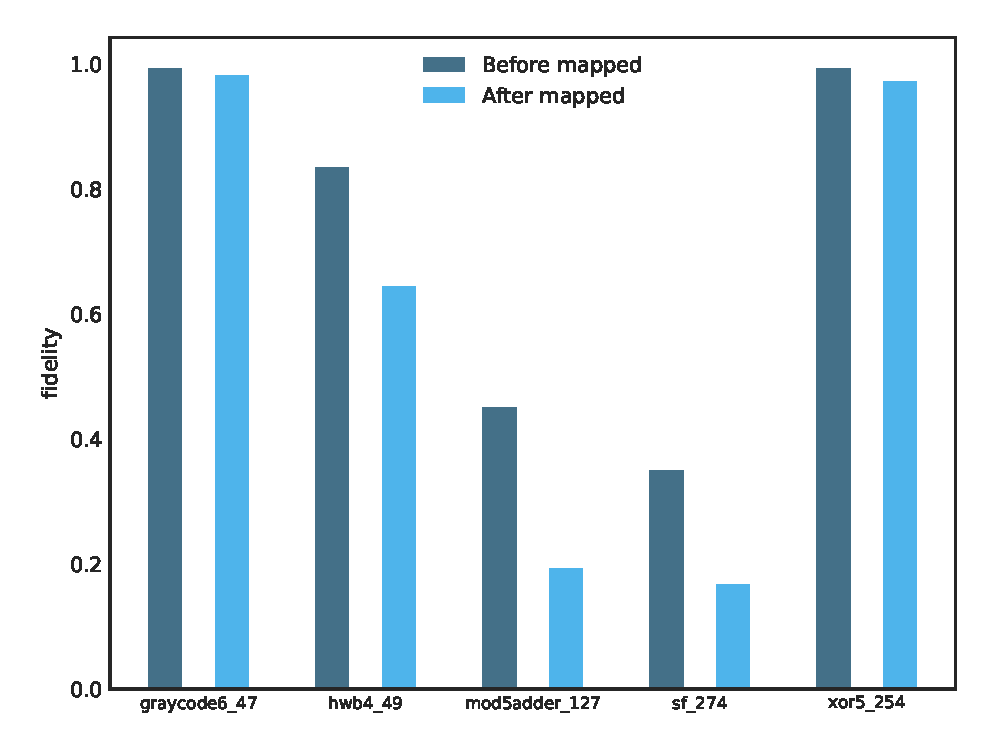
\includegraphics[width=0.7\textwidth]{figures/f_diff_bar_plot.eps}
\caption{\label{fig:f_diff_bar_plot}
Difference of fidelities before and after mapping with the \texttt{minextendrc} router for five different benchmarks.}
\end{figure}

\section{Analysis of the mapping metrics}
\label{sec:org2c64a48}
Once we acknowledged the behaviour of the error growth due to the mapping process, it was the time to understand which circuit parameter affects it the most.
In this section we evaluate the behaviour and quality of the mapping metrics.
From the common ones -- number of SWAPs and depth -- to the ones we proposed -- fidelity, probability of success and Quantum Volume.



First we analyze the probability of success and fidelity correlation.
As expected, our experiments prove that both metrics are highly correlated in a logarithmic fashion.
We also appreciated the fact that the probability of success is always higher than the fidelity.
This could suggest that the measurement is 'correcting' circuit errors colliding the state in the correct result, instead of the wrong one.
It is a 'good' mistake that results in the expected solution.
Nevertheless, this behaviour could be caused by the fact that our algorithms are deterministic.
Another knowledge we inherited from the results is that the closer the values are to 0 the more chaotic and random the values will get.



In Fig. \ref{fig:f_ps_correlation_with_meas_error} we plot the results of the framework in terms of probability of success and fidelity. 
For this figure and the figures from now on in this section, each dot is a different benchmark configuration (see \href{appendix-1.org}{Appendix A}) and the colors represent different decoherence times, blue for 30 \(\mu s\) and orange for 10 \(\mu s\).
As we explained in the \href{quantum_computing.org}{Qubits are faulty} section, the shorter the decoherence time the more errors would appear in our quantum system.
Fig. \ref{fig:f_ps_correlation_with_meas_error} highlights a logarithmic correlation as well as the bias between both metrics, proving the fact that the probability of success is always higher than the fidelity.
For instance, for values around 0.6 in fidelity, the probability of success has a value bigger than 0.7 for the majority of the samples.
This behaviour could be due to the small error rate the measurement has.
Note that for values close to 1, fidelity and probability of success tend to be almost equal and linear, which make sense; if some circuit has almost no error, both metrics will be equally good.
At the same time, the closer the values are to 0, the more spread the samples are, proving the chaotic and random behaviour.
It can be seen that the curvature of the fitting line changes depending on the decoherence time of the system.
For higher error rates -- orange function --, the curve tends to decrease faster; what means that the higher the error rates the less fidelity and probability of success will get the circuits.
The cluster that appears between the 0.9 and 1.0 values is due to the amount of simple benchmarks in the selection, as we previously mentioned.

\begin{figure}[htbp]
\centering
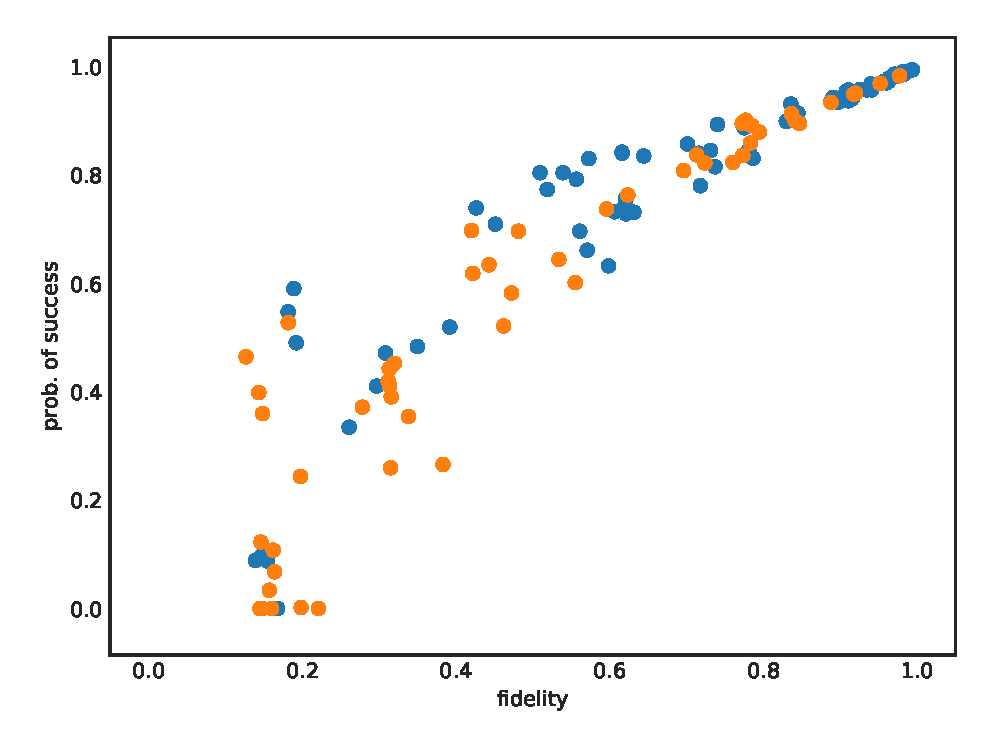
\includegraphics[width=0.7\textwidth]{figures/f_ps_correlation.eps}
\caption{\label{fig:f_ps_correlation_with_meas_error}
Correlation between fidelity and probability of success for two different decoherence times}
\end{figure}



Regarding the rest of the metrics, we analyzed their relation with the fidelity and probability of success.
Instead of using the number of SWAPs we decided to use the number of two-qubit gates because we noticed in the results that the number of gates in the circuit before being mapped are important in this analysis.
For instance, it is not the same to add 10 SWAPs to a circuit with 100 operations than one with 10000.


The results of the main mapping metrics against fidelity are depicted in Fig. \ref{fig:f_metrics_correlation}.
We observe that, for all the cases, the fidelity decreases with an inverse exponential behaviour and that it decreases faster for small decoherence times.
Certainly, the shorter the decoherence times we use the more benchmarks will have non-useful results.
We can also see how fidelity never goes to zero, but it gets constant around 0.2, giving random results.
We consider the point where fidelity is constant as the limit in terms of each of the variables.
We plot a line for the orange samples to mark this point.
Finally, it can be seen how the number of gates is the metric most related with the fidelity; it is the one with the samples more ordered.

\begin{figure}[htbp]
\centering
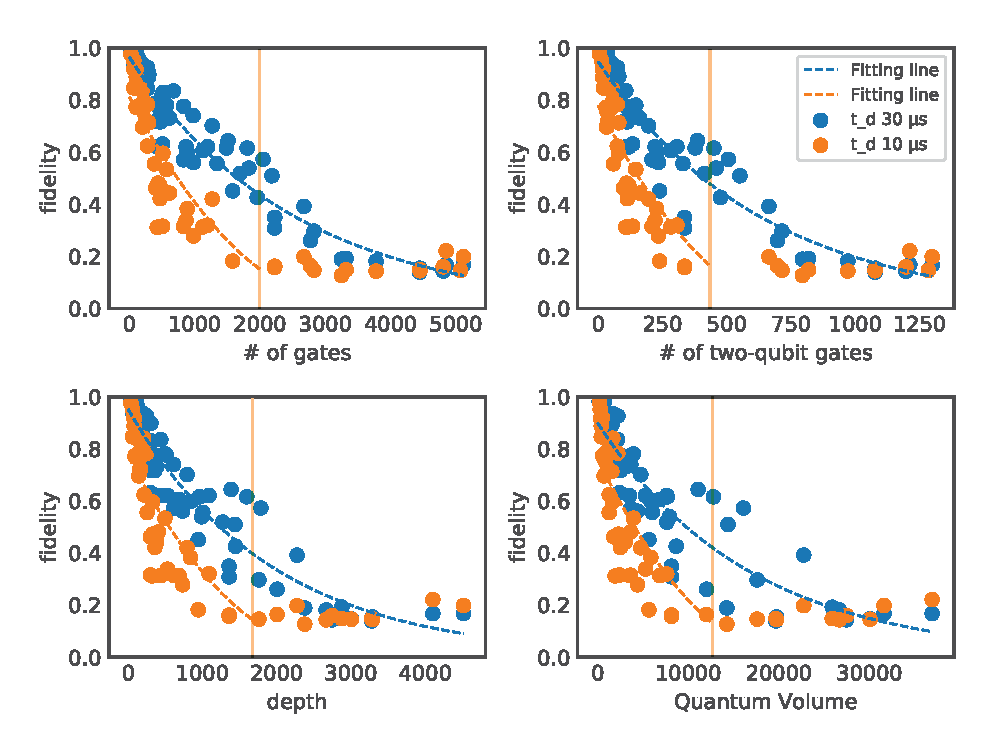
\includegraphics[width=\textwidth]{figures/f_metrics_correlation_poly.eps}
\caption{\label{fig:f_metrics_correlation}
Correlation between fidelity and the mapping metrics.}
\end{figure}

The correlation between the probability of success and the other metrics can be see in Fig. \ref{fig:ps_metrics_correlation}.
We also observe a decreasing behaviour, although the shape is not as clear as in the case of fidelity.
This could be provoked, again, by the final error added by the measurement gate and by the fact that, most of the times, the measurement is correcting the wrong solutions.
The figure also highlights how the fast probability of success decreases depending on the decoherence time.

\begin{figure}[htbp]
\centering
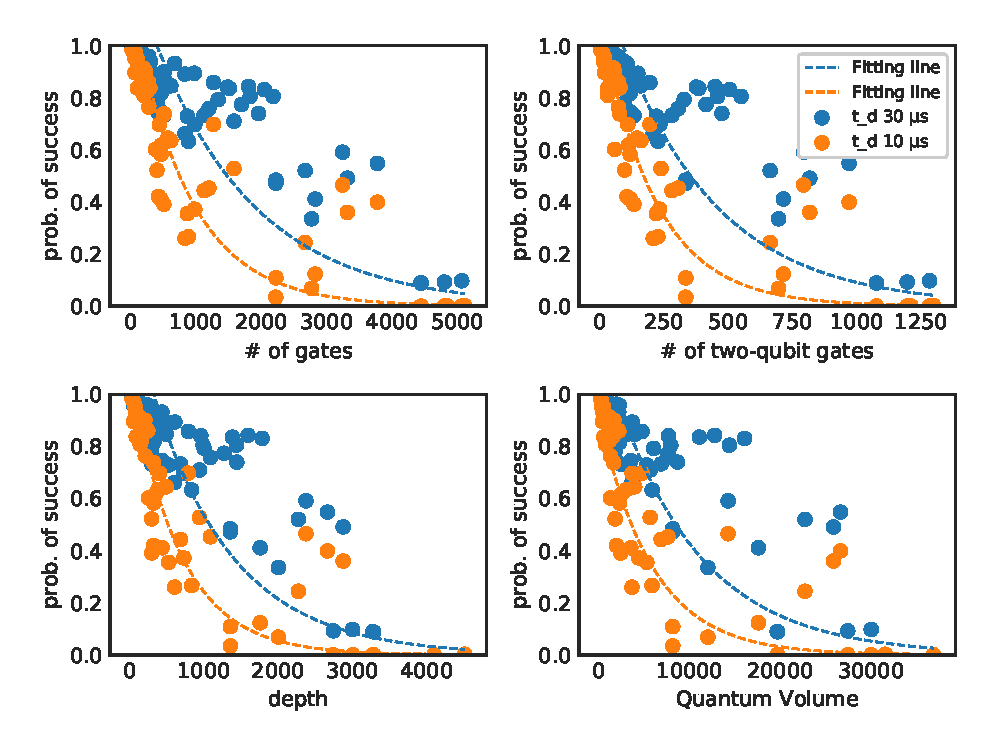
\includegraphics[width=\textwidth]{figures/ps_metrics_correlation.eps}
\caption{\label{fig:ps_metrics_correlation}
Correlation between probability of success and the mapping metrics.}
\end{figure}

We can also see in both figures that, as announced before, there is a cluster of benchmarks with high fidelity and high probability of success.
This happens because of the high concentration of small benchmarks, due to the simulation difficulties.
On the contrary, the rest of the values are a bit spread.
In general, we observe a high correlation between all of the metrics; so in order to get correlation quality values to differ between the metrics, we calculated the Pearson correlation coefficient.
Note that the Pearson coefficient measures linear correlations and, as it will be seen in Fig. \ref{fig:f_metrics_correlation}, the metrics behave in an inverse exponential fashion against fidelity.
For this reason, we applied a \(log\) transformation to our fidelity data in order to make it linear for the Pearson calculation.


As it can be seen in the Pearson values (Tab. \ref{tab:pearson_corr_f} and Tab. \ref{tab:pearson_corr_ps}) the most correlated metric is the number of two-qubit gates.
These results hold the fact that the quality of the mapping depends directly on the longitude of the targeted circuit before it is being mapped.
For example, a long circuit well mapped will have always worse results in fidelity or probability of success than a short circuit badly mapped.
As Tab. \ref{tab:pearson_corr_f} and Tab. \ref{tab:pearson_corr_ps} highlight, we have a worse correlation for the shorter decoherence time.
This lack of correlation can be attributed to the fact that the majority of the samples with \(t_d = 1000\) are highly affected by the errors and, therefore, the samples have more random values.
Moreover, contrary to expectations, the Quantum Volume was the least correlated metric.
This small lack of correlation can be attributed to the imprecise formula that we chose to calculate it.
Future work needs to be done to inspect a better formula.
Finally, if we compare both tables, we can see that the fidelity is more correlated with the metrics that the probability of success.
It is very likely that the reason for this result is that the added measurement error distribution in the end of the circuit adds more noise and spreads our samples.
Also the 'correcting' errors behaviour of the measurement should be taken into account.

\begin{center}
\captionof{table}{\label{tab:pearson_corr_f}
Pearson correlation coefficient of the log transformation of fidelity against the metrics(\(\rho _{log(f),Y}\)), where \(Y\) is one of the four metrics we analyze}
\begin{tabular}{lrrrr}
 & \# of Gates & \# of Two-qubit gates & Depth & \(V_Q\)\\
\hline
\(t_d = 3000\) & -0.9730 & -0.9600 & -0.9455 & -0.9118\\
\(t_d = 1000\) & -0.8466 & -0.8135 & -0.8093 & -0.7736\\
\hline
\end{tabular}
\end{center}

\begin{center}
\captionof{table}{\label{tab:pearson_corr_ps}
Pearson correlation coefficient for the probability of success against the metrics (\(\rho _{p_s,Y}\)), where \(Y\) is one of the four metrics we analyze}
\begin{tabular}{lrrrr}
 & \# of Gates & \# of Two-qubit gates & Depth & \(V_Q\)\\
\hline
\(t_d = 3000\) & -0.9363 & -0.9248 & -0.9179 & -0.8797\\
\(t_d = 1000\) & -0.8341 & -0.8097 & -0.8076 & -0.7686\\
\hline
\end{tabular}
\end{center}
